\subsection{Quicksort}
\textbf{Live-Programmierung}
Wird demnächst bereitgestellt.

\textbf{Tafelanschrieb}
Quicksort hat eine Laufzeit von $\Theta(n \log n)$
\begin{center}
\textbf{Vergleichsbasierte Sortieralgorithmen}\\
\begin{tabular}{c|c}
    \multicolumn{2}{c}{Laufzeit}\\
    $\Theta(n^2)$ & $\Theta(n \log n)$\\
    InsertionSort & Quicksort\\\hline
    BubbleSort & MergeSort\\
     & Heapsort
\end{tabular}
\end{center}
Wir werden zeigen:
\begin{align*}
    \log(n!) = \Theta(n \log n)
\end{align*}


$S_n = $ Menge aller n-Permutationen

\begin{align*}
\sigma \in S_n\\
(\sigma^{-1})^{-1} = \sigma
\begin{array}{|c|c|}\hline
    \sigma(1) & 1\\\hline
    \sigma(2) & 2\\\hline
    \sigma(3) & 3\\\hline
    \vdots & \vdots\\\hline
    \sigma(n) & n\\\hline
\end{array}
\overset{\text{Sortiere}}{\underset{\text{nach der ersten Spalte}}{\longrightarrow}}
\begin{array}{|c|c|}\hline
    1 & \sigma^{-1}(1)\\\hline
    2 & \sigma^{-1}(2)\\\hline
    3 & \sigma^{-1}(3)\\\hline
    \vdots & \vdots\\\hline
    n & \sigma^{-1}(n)\\\hline
\end{array}\\

\sigma: \{1, \dots, n\} \rightarrow \{1, \dots, n\}\\
\text{bijektiv}\\
\sigma^{-1}: \text{Umkehrabbildung}
\end{align*}

\begin{center}
\newcommand{\ersterGraph}{
    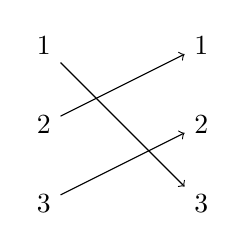
\begin{tikzpicture}
    \node (1) at (0,0) {1};
    \node (2) at (0,-1) {2};
    \node (3) at (0,-2) {3};
    \node (4) at (2,0) {1};
    \node (5) at (2,-1) {2};
    \node (6) at (2,-2) {3};
    \draw[->] (1) to (6);
    \draw[->] (2) to (4);
    \draw[->] (3) to (5);
    \end{tikzpicture}}
\newcommand{\zweiterGraph}{
    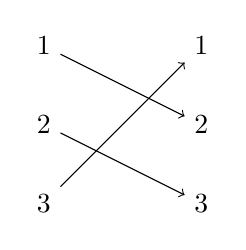
\begin{tikzpicture}
    \node (1) at (0,0) {1};
    \node (2) at (0,-1) {2};
    \node (3) at (0,-2) {3};
    \node (4) at (2,0) {1};
    \node (5) at (2,-1) {2};
    \node (6) at (2,-2) {3};
    \draw[->] (1) to (5);
    \draw[->] (2) to (6);
    \draw[->] (3) to (4);
    \end{tikzpicture}}
    
    \begin{tabular}{cccc}
        $\sigma:$ & \ersterGraph & $\sigma^{-1}$ & \zweiterGraph
    \end{tabular}
\end{center}


\subsection{Beweis des Satzes}
\renewcommand*\circled[1]{\tikz[baseline=(char.base)]{
  \node[shape=circle,draw,inner sep=1pt] (char) {#1};}}
  \renewcommand*\rectangled[1]{\tikz[baseline=(char.base)]{
  \node[shape=rectangle,draw,inner sep=2pt] (char) {#1};}}
Angenommen $T$ ist die erwartete Anzahl von Vergleichen zum Sortieren einer zufälligen n-Permutation. Dann gibt es mindestens $\frac{n!}{2}$ n-Permutationen, für die der Algorithmus $\leq 2 \cdot T$ Vergleiche braucht. Der Algorithmus stellt also $X \leq 2 \cdot T$ Vergleichsanfragen.\\
Die Antworten können durch einen Vektor aus $\{0, +1, -1\}^X$ beschrieben werden. Weil beim Sortiervorgang keine Information verloren geht, folgt:
\[3^{2T + 1} \geq \sum_{X = 1}^{2 \cdot T} 3^X \geq \circled{$\frac{n!}{2}$} \Rightarrow 2T + 1 \geq \log_3(n!) \Rightarrow T \geq \frac{1}{2}\log_3(n!) -1 \Rightarrow T=\rectangled{$\Omega(\log(n!))$}\]
\[\log_3 z = \frac{\log(z)}{\log 3}\]